\chapter{Anhang}
\label{ch:anhang}
\todo{erkläre kurz, warum ich die plots genommen habe}
%% ==============================
%

%%%%%      PERSON 5 LOSO %%%%%%%%%%%%%%%%%%%%%%%
\begin{figure}
    \textbf{Person 5: Random Forest ($w=5\si{\s}$, $d=1\si{\s}$)}
      \centering
      \begin{subfigure}{1\textwidth}
          \includegraphics[width=1\textwidth]{evaluation/loso_5sec/random_forest_loso/Random Forest (Leave one Subject out: Person 5 back).png}
          %\caption{Resultate der Person 6 auf dem Rücken liegend.}
        \end{subfigure}
        \begin{subfigure}{1\textwidth}
          \includegraphics[width=1\textwidth]{evaluation/loso_5sec/random_forest_loso/Random Forest (Leave one Subject out: Person 5 side).png}
          %\caption{Resultate der Person 6 auf der Seite liegend.}
        \end{subfigure}
        \begin{subfigure}{1\textwidth}
          \includegraphics[width=1\textwidth]{evaluation/loso_5sec/random_forest_loso/Random Forest (Leave one Subject out: Person 5 stomach).png}
          %\caption{Resultate der Person 6 auf dem Bauch liegend.}
      \end{subfigure}
        \textbf{Person 5: Random Forest ($w=10\si{\s}$, $d=1\si{\s}$)}
      \centering
      \begin{subfigure}{1\textwidth}
          \includegraphics[width=1\textwidth]{evaluation/loso_10sec/random_forest_loso/Random Forest (Leave one Subject out: Person 5 back).png}
          %\caption{Resultate der Person 6 auf dem Rücken liegend.}
        \end{subfigure}
        \begin{subfigure}{1\textwidth}
          \includegraphics[width=1\textwidth]{evaluation/loso_10sec/random_forest_loso/Random Forest (Leave one Subject out: Person 5 side).png}
          %\caption{Resultate der Person 6 auf der Seite liegend.}
        \end{subfigure}
        \begin{subfigure}{1\textwidth}
          \includegraphics[width=1\textwidth]{evaluation/loso_10sec/random_forest_loso/Random Forest (Leave one Subject out: Person 5 stomach).png}
          %\caption{Resultate der Person 6 auf dem Bauch liegend.}
      \end{subfigure}
  
      %\caption{Das Kreuzvalidierungsverfahren (LOSO) mit dem Klassifikationsalgorithmus XG Boost. Das Modell wurde auf allen Personen, exklusive einer Person trainiert und auf alle Positionen dieser einen Person wurde eine Vorhersage getroffen. Am Beispiel hier sind die Resultate von Person 6 zu sehen. Die blauen Bereiche sind die, in denen die Luft angehalten wurde, die orangene Kurve ist die Vorhersage. ($w=$ Fenstergröße, $d=$ Verschiebung der Fenster)}
      \label{evaluation:xgboost_loso:person6}
\end{figure}
\begin{figure}
    \textbf{Person 5: XG Boost ($w=5\si{\s}$, $d=1\si{\s}$)}
      \centering
      \begin{subfigure}{1\textwidth}
          \includegraphics[width=1\textwidth]{evaluation/loso_5sec/xg_boost_loso/XG Boost (Leave one Subject out: Person 5 back).png}
          %\caption{Resultate der Person 6 auf dem Rücken liegend.}
        \end{subfigure}
        \begin{subfigure}{1\textwidth}
          \includegraphics[width=1\textwidth]{evaluation/loso_5sec/xg_boost_loso/XG Boost (Leave one Subject out: Person 5 side).png}
          %\caption{Resultate der Person 6 auf der Seite liegend.}
        \end{subfigure}
        \begin{subfigure}{1\textwidth}
          \includegraphics[width=1\textwidth]{evaluation/loso_5sec/xg_boost_loso/XG Boost (Leave one Subject out: Person 5 stomach).png}
          %\caption{Resultate der Person 6 auf dem Bauch liegend.}
      \end{subfigure}
        \textbf{Person 5: XG Boost ($w=10\si{\s}$, $d=1\si{\s}$)}
      \centering
      \begin{subfigure}{1\textwidth}
          \includegraphics[width=1\textwidth]{evaluation/loso_10sec/xg_boost_loso/XG Boost (Leave one Subject out: Person 5 back).png}
          %\caption{Resultate der Person 6 auf dem Rücken liegend.}
        \end{subfigure}
        \begin{subfigure}{1\textwidth}
          \includegraphics[width=1\textwidth]{evaluation/loso_10sec/xg_boost_loso/XG Boost (Leave one Subject out: Person 5 side).png}
          %\caption{Resultate der Person 6 auf der Seite liegend.}
        \end{subfigure}
        \begin{subfigure}{1\textwidth}
          \includegraphics[width=1\textwidth]{evaluation/loso_10sec/xg_boost_loso/XG Boost (Leave one Subject out: Person 5 stomach).png}
          %\caption{Resultate der Person 6 auf dem Bauch liegend.}
      \end{subfigure}
  
      %\caption{Das Kreuzvalidierungsverfahren (LOSO) mit dem Klassifikationsalgorithmus XG Boost. Das Modell wurde auf allen Personen, exklusive einer Person trainiert und auf alle Positionen dieser einen Person wurde eine Vorhersage getroffen. Am Beispiel hier sind die Resultate von Person 6 zu sehen. Die blauen Bereiche sind die, in denen die Luft angehalten wurde, die orangene Kurve ist die Vorhersage. ($w=$ Fenstergröße, $d=$ Verschiebung der Fenster)}
      \label{evaluation:xgboost_loso:person6}
\end{figure}

%%%%%      PERSON 5 LOSO %%%%%%%%%%%%%%%%%%%%%%%
\begin{figure}
    \textbf{Person 7: Random Forest ($w=5\si{\s}$, $d=1\si{\s}$)}
      \centering
      \begin{subfigure}{1\textwidth}
          \includegraphics[width=1\textwidth]{evaluation/loso_5sec/random_forest_loso/Random Forest (Leave one Subject out: Person 7 back).png}
          %\caption{Resultate der Person 6 auf dem Rücken liegend.}
        \end{subfigure}
        \begin{subfigure}{1\textwidth}
          \includegraphics[width=1\textwidth]{evaluation/loso_5sec/random_forest_loso/Random Forest (Leave one Subject out: Person 7 side).png}
          %\caption{Resultate der Person 6 auf der Seite liegend.}
        \end{subfigure}
        \begin{subfigure}{1\textwidth}
          \includegraphics[width=1\textwidth]{evaluation/loso_5sec/random_forest_loso/Random Forest (Leave one Subject out: Person 7 stomach).png}
          %\caption{Resultate der Person 6 auf dem Bauch liegend.}
      \end{subfigure}
        \textbf{Person 7: Random Forest ($w=10\si{\s}$, $d=1\si{\s}$)}
      \centering
      \begin{subfigure}{1\textwidth}
          \includegraphics[width=1\textwidth]{evaluation/loso_10sec/random_forest_loso/Random Forest (Leave one Subject out: Person 7 back).png}
          %\caption{Resultate der Person 6 auf dem Rücken liegend.}
        \end{subfigure}
        \begin{subfigure}{1\textwidth}
          \includegraphics[width=1\textwidth]{evaluation/loso_10sec/random_forest_loso/Random Forest (Leave one Subject out: Person 7 side).png}
          %\caption{Resultate der Person 6 auf der Seite liegend.}
        \end{subfigure}
        \begin{subfigure}{1\textwidth}
          \includegraphics[width=1\textwidth]{evaluation/loso_10sec/random_forest_loso/Random Forest (Leave one Subject out: Person 7 stomach).png}
          %\caption{Resultate der Person 6 auf dem Bauch liegend.}
      \end{subfigure}
  
      %\caption{Das Kreuzvalidierungsverfahren (LOSO) mit dem Klassifikationsalgorithmus XG Boost. Das Modell wurde auf allen Personen, exklusive einer Person trainiert und auf alle Positionen dieser einen Person wurde eine Vorhersage getroffen. Am Beispiel hier sind die Resultate von Person 6 zu sehen. Die blauen Bereiche sind die, in denen die Luft angehalten wurde, die orangene Kurve ist die Vorhersage. ($w=$ Fenstergröße, $d=$ Verschiebung der Fenster)}
      \label{evaluation:xgboost_loso:person6}
\end{figure}
\begin{figure}
    \textbf{Person 7: XG Boost ($w=5\si{\s}$, $d=1\si{\s}$)}
      \centering
      \begin{subfigure}{1\textwidth}
          \includegraphics[width=1\textwidth]{evaluation/loso_5sec/xg_boost_loso/XG Boost (Leave one Subject out: Person 7 back).png}
          %\caption{Resultate der Person 6 auf dem Rücken liegend.}
        \end{subfigure}
        \begin{subfigure}{1\textwidth}
          \includegraphics[width=1\textwidth]{evaluation/loso_5sec/xg_boost_loso/XG Boost (Leave one Subject out: Person 7 side).png}
          %\caption{Resultate der Person 6 auf der Seite liegend.}
        \end{subfigure}
        \begin{subfigure}{1\textwidth}
          \includegraphics[width=1\textwidth]{evaluation/loso_5sec/xg_boost_loso/XG Boost (Leave one Subject out: Person 7 stomach).png}
          %\caption{Resultate der Person 6 auf dem Bauch liegend.}
      \end{subfigure}
        \textbf{Person 7: XG Boost ($w=10\si{\s}$, $d=1\si{\s}$)}
      \centering
      \begin{subfigure}{1\textwidth}
          \includegraphics[width=1\textwidth]{evaluation/loso_10sec/xg_boost_loso/XG Boost (Leave one Subject out: Person 7 back).png}
          %\caption{Resultate der Person 6 auf dem Rücken liegend.}
        \end{subfigure}
        \begin{subfigure}{1\textwidth}
          \includegraphics[width=1\textwidth]{evaluation/loso_10sec/xg_boost_loso/XG Boost (Leave one Subject out: Person 7 side).png}
          %\caption{Resultate der Person 6 auf der Seite liegend.}
        \end{subfigure}
        \begin{subfigure}{1\textwidth}
          \includegraphics[width=1\textwidth]{evaluation/loso_10sec/xg_boost_loso/XG Boost (Leave one Subject out: Person 7 stomach).png}
          %\caption{Resultate der Person 6 auf dem Bauch liegend.}
      \end{subfigure}
  
      %\caption{Das Kreuzvalidierungsverfahren (LOSO) mit dem Klassifikationsalgorithmus XG Boost. Das Modell wurde auf allen Personen, exklusive einer Person trainiert und auf alle Positionen dieser einen Person wurde eine Vorhersage getroffen. Am Beispiel hier sind die Resultate von Person 6 zu sehen. Die blauen Bereiche sind die, in denen die Luft angehalten wurde, die orangene Kurve ist die Vorhersage. ($w=$ Fenstergröße, $d=$ Verschiebung der Fenster)}
      \label{evaluation:xgboost_loso:person6}
\end{figure}

%%%%%      PERSON 8 LOSO %%%%%%%%%%%%%%%%%%%%%%%
\begin{figure}
    \textbf{Person 8: Random Forest ($w=5\si{\s}$, $d=1\si{\s}$)}
      \centering
      \begin{subfigure}{1\textwidth}
          \includegraphics[width=1\textwidth]{evaluation/loso_5sec/random_forest_loso/Random Forest (Leave one Subject out: Person 8 back).png}
          %\caption{Resultate der Person 6 auf dem Rücken liegend.}
        \end{subfigure}
        \begin{subfigure}{1\textwidth}
          \includegraphics[width=1\textwidth]{evaluation/loso_5sec/random_forest_loso/Random Forest (Leave one Subject out: Person 8 side).png}
          %\caption{Resultate der Person 6 auf der Seite liegend.}
        \end{subfigure}
        \begin{subfigure}{1\textwidth}
          \includegraphics[width=1\textwidth]{evaluation/loso_5sec/random_forest_loso/Random Forest (Leave one Subject out: Person 8 stomach).png}
          %\caption{Resultate der Person 6 auf dem Bauch liegend.}
      \end{subfigure}
        \textbf{Person 8: Random Forest ($w=10\si{\s}$, $d=1\si{\s}$)}
      \centering
      \begin{subfigure}{1\textwidth}
          \includegraphics[width=1\textwidth]{evaluation/loso_10sec/random_forest_loso/Random Forest (Leave one Subject out: Person 8 back).png}
          %\caption{Resultate der Person 6 auf dem Rücken liegend.}
        \end{subfigure}
        \begin{subfigure}{1\textwidth}
          \includegraphics[width=1\textwidth]{evaluation/loso_10sec/random_forest_loso/Random Forest (Leave one Subject out: Person 8 side).png}
          %\caption{Resultate der Person 6 auf der Seite liegend.}
        \end{subfigure}
        \begin{subfigure}{1\textwidth}
          \includegraphics[width=1\textwidth]{evaluation/loso_10sec/random_forest_loso/Random Forest (Leave one Subject out: Person 8 stomach).png}
          %\caption{Resultate der Person 6 auf dem Bauch liegend.}
      \end{subfigure}
  
      %\caption{Das Kreuzvalidierungsverfahren (LOSO) mit dem Klassifikationsalgorithmus XG Boost. Das Modell wurde auf allen Personen, exklusive einer Person trainiert und auf alle Positionen dieser einen Person wurde eine Vorhersage getroffen. Am Beispiel hier sind die Resultate von Person 6 zu sehen. Die blauen Bereiche sind die, in denen die Luft angehalten wurde, die orangene Kurve ist die Vorhersage. ($w=$ Fenstergröße, $d=$ Verschiebung der Fenster)}
      \label{evaluation:xgboost_loso:person6}
\end{figure}
\begin{figure}
    \textbf{Person 8: XG Boost ($w=5\si{\s}$, $d=1\si{\s}$)}
      \centering
      \begin{subfigure}{1\textwidth}
          \includegraphics[width=1\textwidth]{evaluation/loso_5sec/xg_boost_loso/XG Boost (Leave one Subject out: Person 8 back).png}
          %\caption{Resultate der Person 6 auf dem Rücken liegend.}
        \end{subfigure}
        \begin{subfigure}{1\textwidth}
          \includegraphics[width=1\textwidth]{evaluation/loso_5sec/xg_boost_loso/XG Boost (Leave one Subject out: Person 8 side).png}
          %\caption{Resultate der Person 6 auf der Seite liegend.}
        \end{subfigure}
        \begin{subfigure}{1\textwidth}
          \includegraphics[width=1\textwidth]{evaluation/loso_5sec/xg_boost_loso/XG Boost (Leave one Subject out: Person 8 stomach).png}
          %\caption{Resultate der Person 6 auf dem Bauch liegend.}
      \end{subfigure}
        \textbf{Person 8: XG Boost ($w=10\si{\s}$, $d=1\si{\s}$)}
      \centering
      \begin{subfigure}{1\textwidth}
          \includegraphics[width=1\textwidth]{evaluation/loso_10sec/xg_boost_loso/XG Boost (Leave one Subject out: Person 8 back).png}
          %\caption{Resultate der Person 6 auf dem Rücken liegend.}
        \end{subfigure}
        \begin{subfigure}{1\textwidth}
          \includegraphics[width=1\textwidth]{evaluation/loso_10sec/xg_boost_loso/XG Boost (Leave one Subject out: Person 8 side).png}
          %\caption{Resultate der Person 6 auf der Seite liegend.}
        \end{subfigure}
        \begin{subfigure}{1\textwidth}
          \includegraphics[width=1\textwidth]{evaluation/loso_10sec/xg_boost_loso/XG Boost (Leave one Subject out: Person 8 stomach).png}
          %\caption{Resultate der Person 6 auf dem Bauch liegend.}
      \end{subfigure}
  
      %\caption{Das Kreuzvalidierungsverfahren (LOSO) mit dem Klassifikationsalgorithmus XG Boost. Das Modell wurde auf allen Personen, exklusive einer Person trainiert und auf alle Positionen dieser einen Person wurde eine Vorhersage getroffen. Am Beispiel hier sind die Resultate von Person 6 zu sehen. Die blauen Bereiche sind die, in denen die Luft angehalten wurde, die orangene Kurve ist die Vorhersage. ($w=$ Fenstergröße, $d=$ Verschiebung der Fenster)}
      \label{evaluation:xgboost_loso:person6}
\end{figure}

%%%%%      PERSON 5 LOSO %%%%%%%%%%%%%%%%%%%%%%%
\begin{figure}
    \textbf{Person 5 (nur einzelne Positionen): Random Forest ($w=5\si{\s}$, $d=1\si{\s}$)}
      \centering
      \begin{subfigure}{1\textwidth}
          \includegraphics[width=1\textwidth]{evaluation/loso_5sec/random_forest_loso_back_prediction/Random Forest (Leave one Subject out, only back data: Person 5).png}
          %\caption{Resultate der Person 6 auf dem Rücken liegend.}
        \end{subfigure}
        \begin{subfigure}{1\textwidth}
          \includegraphics[width=1\textwidth]{evaluation/loso_5sec/random_forest_loso_side_prediction/Random Forest (Leave one Subject out, only side data: Person 5).png}
          %\caption{Resultate der Person 6 auf der Seite liegend.}
        \end{subfigure}
        \begin{subfigure}{1\textwidth}
          \includegraphics[width=1\textwidth]{evaluation/loso_5sec/random_forest_loso_stomach_prediction/Random Forest (Leave one Subject out, only stomach data: Person 5).png}
          %\caption{Resultate der Person 6 auf dem Bauch liegend.}
      \end{subfigure}
        \textbf{Person 5 (nur einzelne Positionen): XGBoost ($w=5\si{\s}$, $d=1\si{\s}$)}
      \centering
      \begin{subfigure}{1\textwidth}
          \includegraphics[width=1\textwidth]{evaluation/loso_5sec/xg_boost_loso_back_prediction/XG Boost (Leave one Subject out, only back data: Person 5).png}
          %\caption{Resultate der Person 6 auf dem Rücken liegend.}
        \end{subfigure}
        \begin{subfigure}{1\textwidth}
            \includegraphics[width=1\textwidth]{evaluation/loso_5sec/xg_boost_loso_side_prediction/XG Boost (Leave one Subject out, only side data: Person 5).png}
          %\caption{Resultate der Person 6 auf der Seite liegend.}
        \end{subfigure}
        \begin{subfigure}{1\textwidth}
            \includegraphics[width=1\textwidth]{evaluation/loso_5sec/xg_boost_loso_stomach_prediction/XG Boost (Leave one Subject out, only stomach data: Person 5).png}
          %\caption{Resultate der Person 6 auf dem Bauch liegend.}
      \end{subfigure}
  
      %\caption{Das Kreuzvalidierungsverfahren (LOSO) mit dem Klassifikationsalgorithmus XG Boost. Das Modell wurde auf allen Personen, exklusive einer Person trainiert und auf alle Positionen dieser einen Person wurde eine Vorhersage getroffen. Am Beispiel hier sind die Resultate von Person 6 zu sehen. Die blauen Bereiche sind die, in denen die Luft angehalten wurde, die orangene Kurve ist die Vorhersage. ($w=$ Fenstergröße, $d=$ Verschiebung der Fenster)}
      \label{evaluation:xgboost_loso:person6}
\end{figure}
\begin{figure}
    \textbf{Person 5 (nur einzelne Positionen): Random Forest ($w=10\si{\s}$, $d=1\si{\s}$)}
      \centering
      \begin{subfigure}{1\textwidth}
          \includegraphics[width=1\textwidth]{evaluation/loso_10sec/random_forest_loso_back_prediction/Random Forest (Leave one Subject out, only back data: Person 5).png}
          %\caption{Resultate der Person 6 auf dem Rücken liegend.}
        \end{subfigure}
        \begin{subfigure}{1\textwidth}
          \includegraphics[width=1\textwidth]{evaluation/loso_10sec/random_forest_loso_side_prediction/Random Forest (Leave one Subject out, only side data: Person 5).png}
          %\caption{Resultate der Person 6 auf der Seite liegend.}
        \end{subfigure}
        \begin{subfigure}{1\textwidth}
          \includegraphics[width=1\textwidth]{evaluation/loso_10sec/random_forest_loso_stomach_prediction/Random Forest (Leave one Subject out, only stomach data: Person 5).png}
          %\caption{Resultate der Person 6 auf dem Bauch liegend.}
      \end{subfigure}
        \textbf{Person 5 (nur einzelne Positionen): XGBoost ($w=10\si{\s}$, $d=1\si{\s}$)}
      \centering
      \begin{subfigure}{1\textwidth}
          \includegraphics[width=1\textwidth]{evaluation/loso_10sec/xg_boost_loso_back_prediction/XG Boost (Leave one Subject out, only back data: Person 5).png}
          %\caption{Resultate der Person 6 auf dem Rücken liegend.}
        \end{subfigure}
        \begin{subfigure}{1\textwidth}
            \includegraphics[width=1\textwidth]{evaluation/loso_10sec/xg_boost_loso_side_prediction/XG Boost (Leave one Subject out, only side data: Person 5).png}
          %\caption{Resultate der Person 6 auf der Seite liegend.}
        \end{subfigure}
        \begin{subfigure}{1\textwidth}
            \includegraphics[width=1\textwidth]{evaluation/loso_10sec/xg_boost_loso_stomach_prediction/XG Boost (Leave one Subject out, only stomach data: Person 5).png}
          %\caption{Resultate der Person 6 auf dem Bauch liegend.}
      \end{subfigure}
  
      %\caption{Das Kreuzvalidierungsverfahren (LOSO) mit dem Klassifikationsalgorithmus XG Boost. Das Modell wurde auf allen Personen, exklusive einer Person trainiert und auf alle Positionen dieser einen Person wurde eine Vorhersage getroffen. Am Beispiel hier sind die Resultate von Person 6 zu sehen. Die blauen Bereiche sind die, in denen die Luft angehalten wurde, die orangene Kurve ist die Vorhersage. ($w=$ Fenstergröße, $d=$ Verschiebung der Fenster)}
      \label{evaluation:xgboost_loso:person6}
\end{figure}